\documentclass{beamer}

\usepackage[T1]{fontenc}
\usepackage[utf8]{inputenc}
\usepackage[ngerman]{babel}

% Schriftart
\usepackage{mathptmx}
\usepackage[scaled=.90]{helvet}
\usepackage{courier}
\usepackage{verbatim}   % useful for program listings

\usepackage{tikz}
\usetikzlibrary{arrows, shapes.arrows}

% Design wählen
\usetheme[secheader]{Boadilla}

\useinnertheme{rectangles} % Vierecke
\setbeamercovered{invisible} % verdeckten Text komplett ausblenden.

% weitere Einstellungen
\setbeamertemplate{mini frames}[box] % shows small rectangles as mini frames.
%\setbeamersize{text margin left=2em,text margin right=2em}
\setbeamertemplate{sections/subsections in toc}[square]
\setbeamertemplate{bibliography item}[default]
\setbeamertemplate{itemize items}[triangle]
\setbeamertemplate{enumerate items}[square]
\setbeamertemplate{blocks}[rounded][shadow=false]

% Navigation ausblenden
\beamertemplatenavigationsymbolsempty

% Nummerierung bei frame breaks
\setbeamertemplate{frametitle continuation}{(\insertcontinuationcount)}

% Trennfolie vor jedem neuen Kapitel
\AtBeginSection{
  \begin{frame}
    \begin{center}
      \structure{\huge \textsf{\insertsection}}
    \end{center}
  \end{frame}
}

% Zentrierung innerhalb einer Aufzählung
\def\MLine#1{\par\hspace*{-\leftmargin}\parbox{\textwidth}{\[#1\]}}
\def\CLine#1{\par\hspace*{-\leftmargin}\parbox{\textwidth}{#1}}

\title[Extraktion von Entitäten aus Suchergebnisseiten]{Extraktion von Entitäten aus Suchergebnisseiten}
\subtitle{Arbeitsgruppe Informationssysteme}
%\author{GRUPPENBEZEICHNUNG\_kurz}
\institute[Arbeitsgruppe Informationssysteme]{
  Universität Duisburg-Essen\\
  Fakultät für Ingenieurwissenschaften\\
  Abteilung Informatik und Angewandte Kognitionswissenschaft\\
  Arbeitsgruppe Informationssysteme 
}
\date{XX.\,Mai 2015}


\begin{document}
  \maketitle

  \begin{frame}[c]{Übersicht}
    \hfill
    \parbox[t][.55\textheight][c]{0.95\textwidth}{%
      \centering %%% oder vergleichbares
      \tableofcontents
    }
  \end{frame}
  
  \section{Aufgabenstellung}
  \begin{frame}[c]{Heutiger Stand}
  \begin{itemize}
  \item Suchmaschinen bieten keine Übersicht über die gefundene Webseiten.
  \item Die Ergebnismenge besteht aus unstrukturierten Daten.
  \item Es findet keine Extraktion von Entitäten statt.
  \end{itemize}
  Alle diese Faktoren führen dazu, dass der Benutzer alle vorgeschlagene Ergebnisse durchsuchen muss, was eine negative Auswirkung auf Benutzerfreundlichkeit und Suchqualität hat.
  \end{frame}
  
  \begin{frame}[c]{Aufgabenstellung}
  Es soll ein Framework entwickelt werden, der
  \begin{itemize}
  \item Die Extraktion von Entitäten aus deutschen Texten ermöglicht.
  \item Die extrahierte Entitäten mit den Daten aus DBpedia verlinkt.
  \item Die verlinkte Entitäten mithilfe von einem API anderen Programmen zur Verfügung stellt
  \end{itemize}
  Der Zweite Schritt lässt uns eine Ontologie aufzubauen, und der letzte Schritt gibt uns die Möglichkeit, verschiedene Benutzerinterfaces zur Datenvisualisierung zu verwenden.
  \end{frame}
  \section{Lösungskonzept}
  \begin{frame}[c]{Kommunikationsdiagramm}
  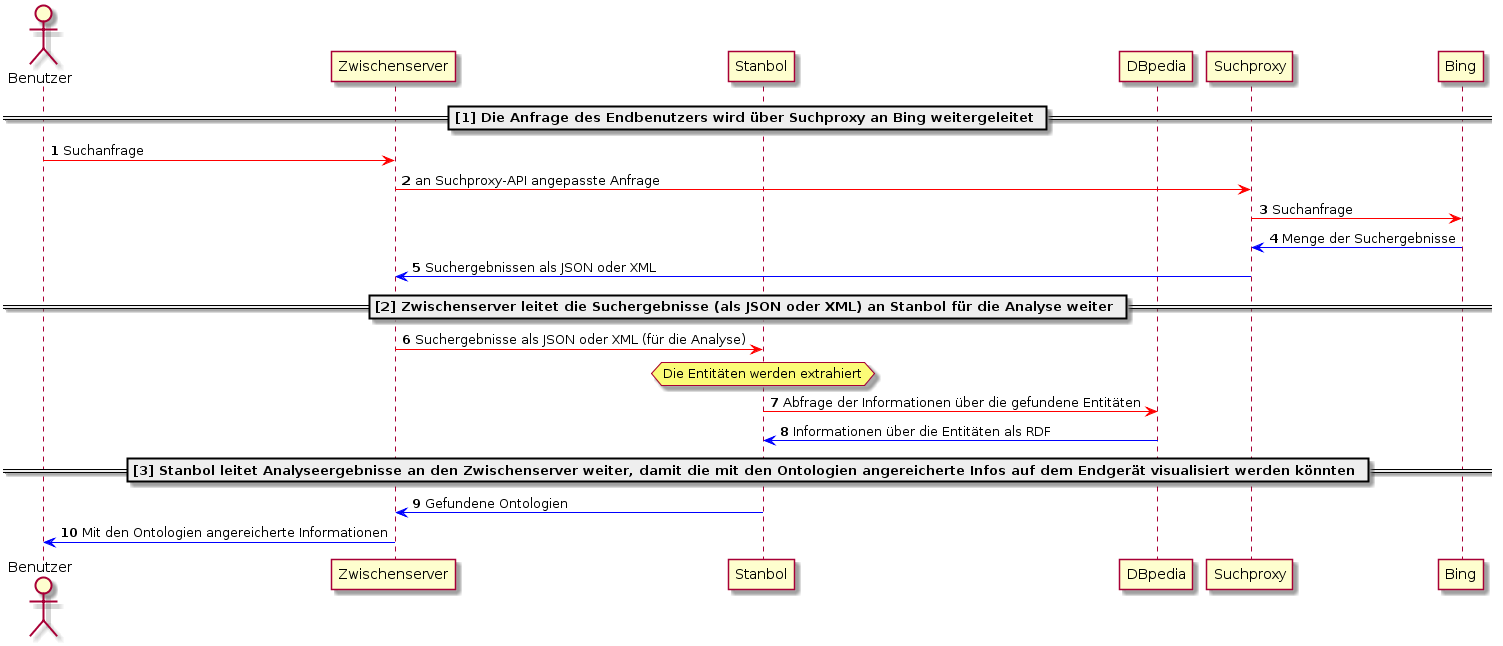
\includegraphics[width=0.94\linewidth]{diagramms/kommunikation.png}
  \end{frame}
  
  \begin{frame}[c]{Funktionsdiagramm des Enchancers}
  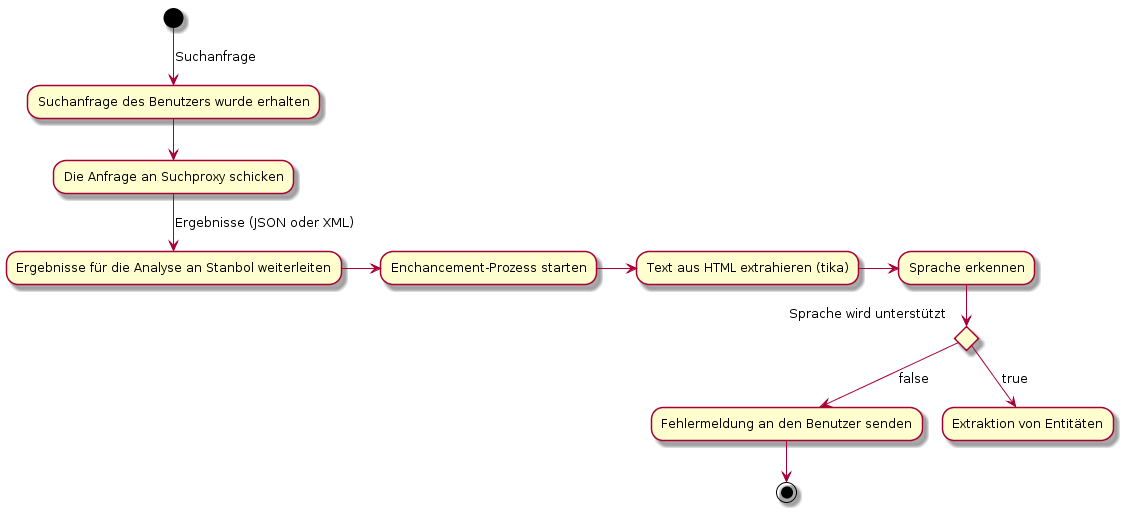
\includegraphics[width=0.4\linewidth]{diagramms/funktionsweise.png}
  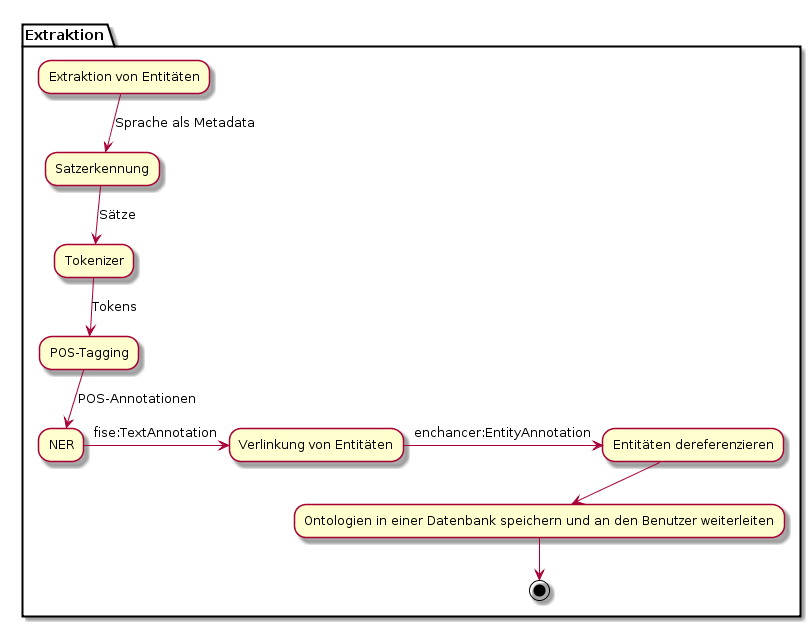
\includegraphics[width=0.5\linewidth]{diagramms/funktionsweise-extraktion.png}
  \end{frame}
  \section{Zeitplan}
  \section{Zusammenfassung}
\end{document}
